
The environment used in the course to run code is the web-based application called JupyterLab, whose document format is the Jupyter Notebook \cite{Kluyver2016jupyter}.
As shown by the figure \ref{fig:jupyter} these documents are divided in an arbitrary number of independent sections called cells that can contain executable code of some programming language, being Python one of the possible ones, or either annotations.

\begin{figure}[!ht]
	\centering
	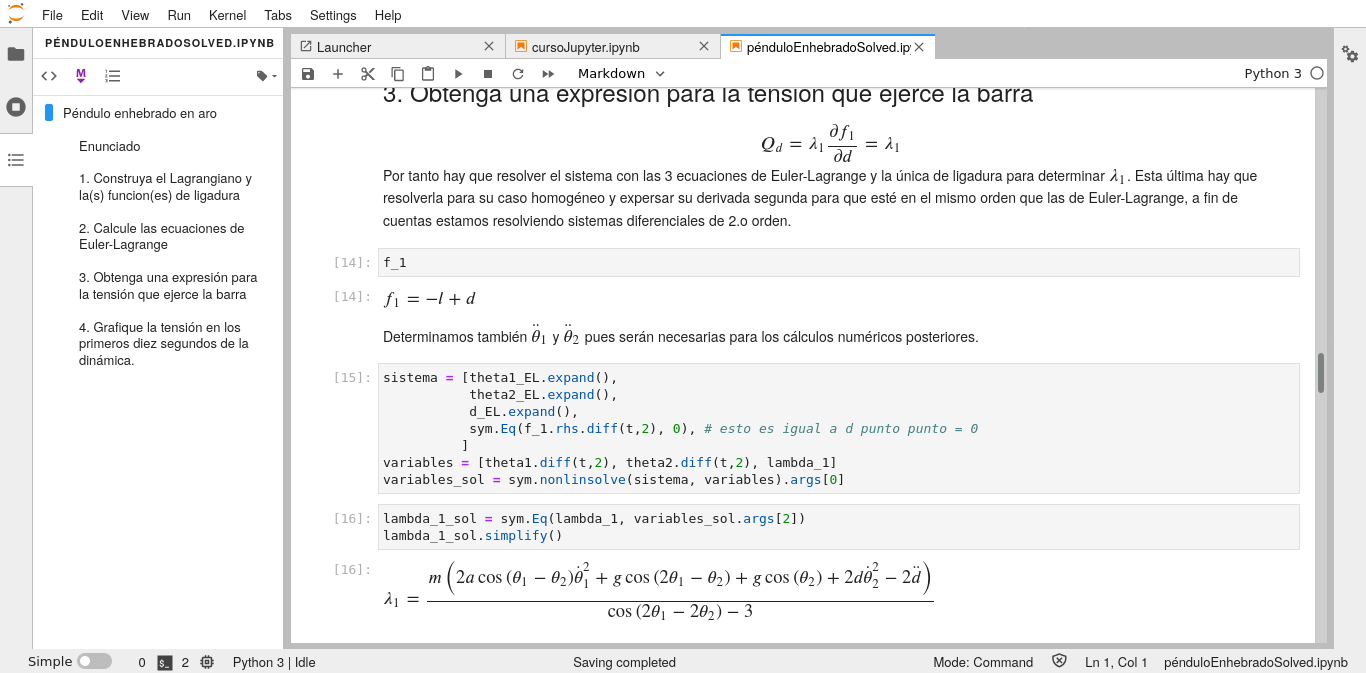
\includegraphics[width=\linewidth]{figuras/screenshot_JupyterLab.png}
	\caption{
		A Jupyter notebook is a set of cells
        containing either exectuable or Markdown code.
		The former can contain text, mathematical expressions or multimedia content.
		The latter are lines of code in various programming languages.
		Interspersing titles in Markdown cells generates the index (on the left) that facilitates location within the document.
	}
	\label{fig:jupyter}
\end{figure}

Annotations cells are written in the Markdown markup language \cite{markdown} that allows to embed text and mathematical expressions in \LaTeX\ format interspersed as well as multimedia content such as web links, images, video and sound players.
The use of \LaTeX\ syntax for the mathematical symbology provides a standardised and clear notation under the guidelines of the American Mathematical Society \cite{ams}. 
This is a further advantage of the Jupyter Notebook as the media for lessons over the blackboard or slides prepared with software such as Microsoft Powerpoint.


% \subsection{Running Jupyter Online}
Students are not required to install any special software on their computer to work with Jupyter Notebooks, only a standard web browser is neeeded to use online services that run Jupyter Notebooks.
This can be an installation of JupyterHub from the Jupyter Project on university-owned servers or commercial clouds, or alternatively one of the services that offer even free alternatives such as CoCalc, IBM Watson or Google Colaboratory\footnote{The authors do no endorse any of the products or services listed here or later in this work that are mentioned only in an informative way.}.
The later, colloquialy known as Colab, is currently in use by the course as it conveniently presents the ability to run notebooks hosted by the online service GitHub.  
A modification in the URL that points to the notebook leads a web browser to open it in Colab. \cite{vallejo_google_2022,google_llc_using_2021}.
Which can be worked on concurrently by students and teachers.
Students are encouraged to collectively solve exercises using this functionality.
As shown by figure \ref{fig:colab}, comments can also be included, an useful feature to correct exercises since the location of errors in the code can be indicated.
The teaching staff can also include inline helping code and new sections into the students notebook.

\begin{figure}[!ht]
	\centering
	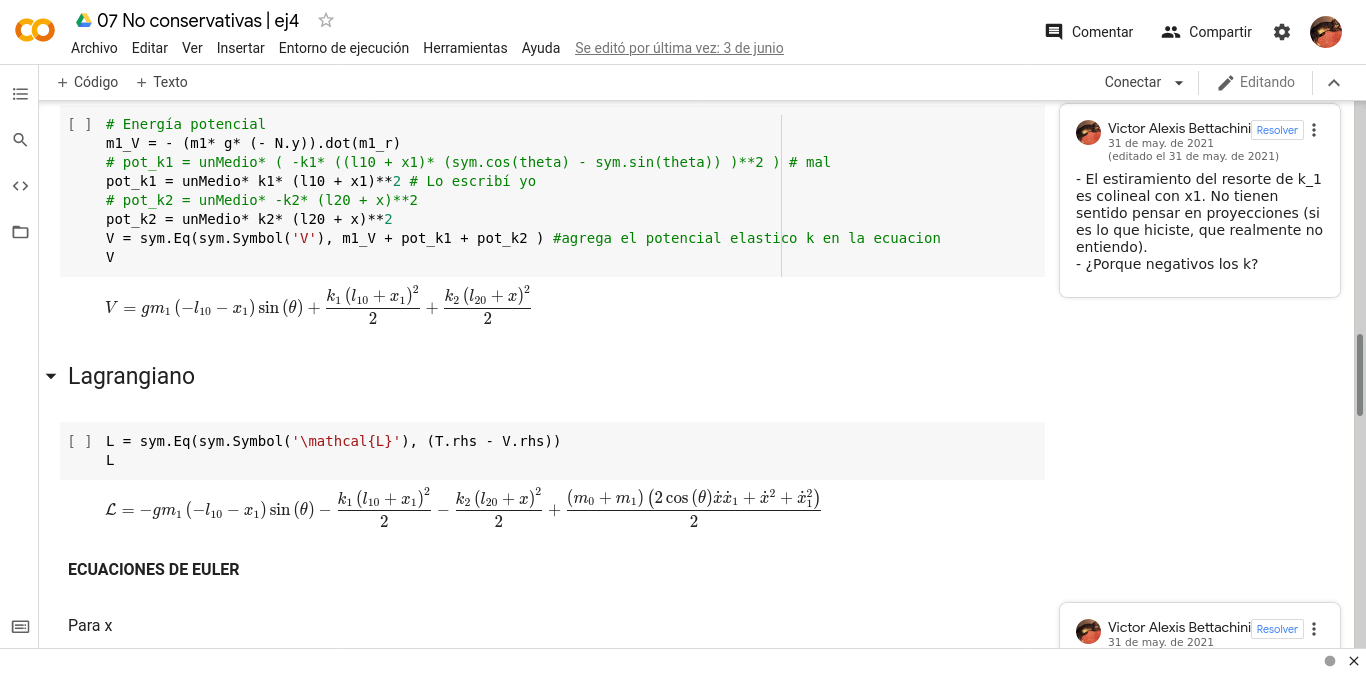
\includegraphics[width=\linewidth]{figuras/comentariosColab.png}
	\caption{
		The Google Colaboratoy website allows Jupyter notebooks to be edited and run concurrently between students and teachers, as well as including comments.
		The latter feature is useful for corrections.
	}
	\label{fig:colab}
\end{figure}